
\section{Introduction}
\label{sec:intro}

\begin{figure}[t]
  \begin{center}
    
\includegraphics[width=0.95\columnwidth]{figs/workflow.eps}
    \caption{Workflow}
    \label{fig:Normal workflow for most multi-tier service oriented systems}
  \end{center}
\end{figure}

\begin{figure*}[t]
  \begin{center}
    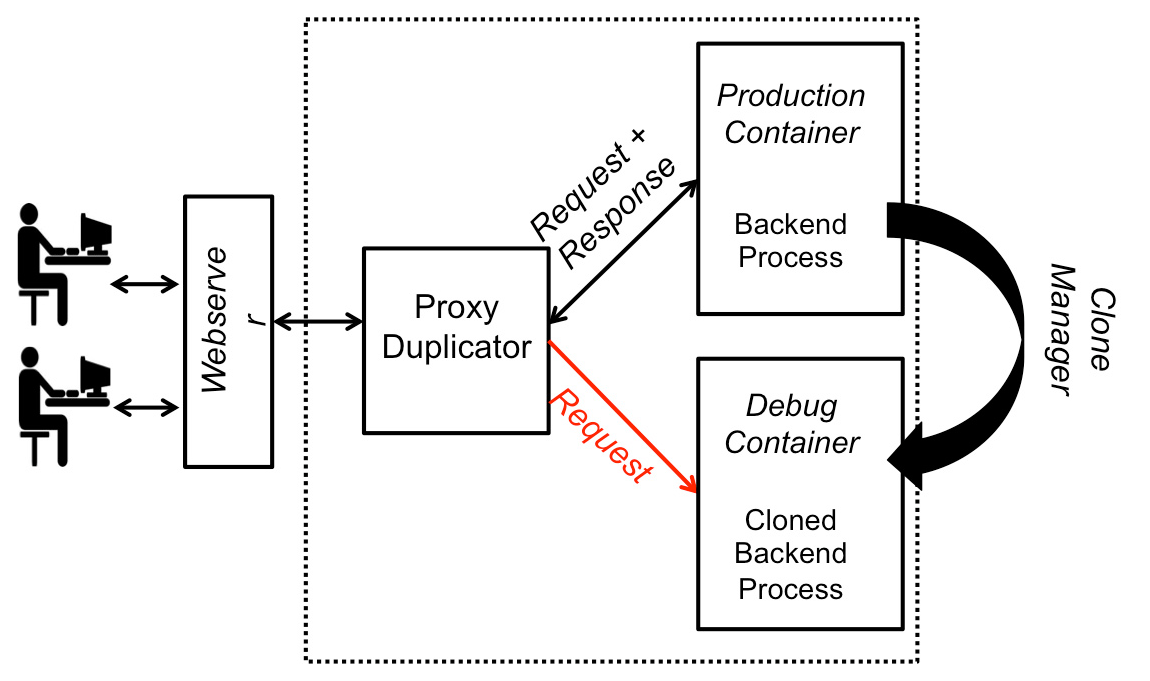
\includegraphics[width=0.8\textwidth]{figs/workflow2.eps}
    \caption{Workflow}
    \label{fig:Backend wrapped around with Parakishan Run-time}
  \end{center}
\end{figure*}

As application software grows and gets more complicated, testing large scale applications has become increasingly important. 
However, it is often impossible to recreate realistic workloads in an offline development environment for large scale multi-tier or cloud based applications.
On the other hand, there has been an equally impressive increase in the scale of computing resources, and distributed scalability of infrastructure.
This often allows for redundant computation, which can be used for testing purposes. 
Leveraging this abundance of resource we present a testing harness which allows the user to dynamically insert test cases in a production environment( we call this in-vivo testing).

We have designed a tool called \texttt{Parikshan}\footnote{Parikshan is the sanskrit word for testing}, which allows capturing the context of application, and allows for a test-case to be run without effecting the sanctity/and performance of the actual application. 
This is done by cloning a production server and creating two containers: a production container, and a testing container. 
We duplicate the incoming traffic to both the production container and the test container using a custom proxy, which ignores the responses from the test-container. 
The testing on the test-container is done on the fly using dynamic instrumentation, hence any set of test-cases can be turned on whenever required. 
%This is achieved by using dynamic instrumentation mechanisms to clone a VM by forking off from a running executed state and encapsulating the forked execution in a VM.
The user can pre-define probe points for dynamically inserting test-cases (by default the entry and exit of each function is considered a probe point).
Since the test is executed in a VM it acts like a sandbox which restricts it from causing any perturbation to the state of the parent process, or effecting the sanity of the responses to the production client. 
We synchronize the production and test containers using a variant of live migration without suspending the services of the production server. 
Frequent synchronization is necessary because the test container can potentially go out of sync with the production because of non-determinism or because a test-case changes the state of the container, and effects future problems. 


The key contributions of this paper are:

\begin{itemize}
\item Our tool provides a sandbox environment to execute test cases in the production environment. 
This allows for a safe and secure test harness which does not effect the production state, and allows the application to proceed in it's execution.
\item We allow for dynamic insertion of the test case, and safetly capturing the context of the application. Dynamically inserting test-cases is important to avoid relaunching binaries in the test-container with the required test-cases. 
Restarting binaries is not possible, because it would break active network connections, and destroy the state of the test container
%\texttt{Zero-Probe Effect} probe points are added to the application which can be activated to insert test cases using ptrace\cite{ptrace}.
%The use of dynamic instrumentation capability to add test cases in an application is an extension of our previous work of a dynamic instrumentation tool iProbe \cite{iProbe}
\end{itemize}

%The authors previous work in in-vivo testing\cite{invite} explored testing in the wild by initiating test cases in the production environment and sharing the load across several instances of deployed application.
%This approach adds test-cases in predetermined functions before starting the execution of the process, and periodically executes them in the run-time environment based on a probabilistic function. 

%\cite{dapper}

\subsection{Contributions}
\label{sec:contributions}

The impact of sandbox testing can be seen in several different ways

\begin{itemize}
  \item \textbf{Sandbox Live Testing}
    One of the key motivations leading to \emph{Parikshan} is to provide a harness to allow the user to test real, live implementations. 


  \item \textbf{Fault Tolerance}
  \item \textbf{Verification}
  \item \textbf{Integration Testing}
\end{itemize}

